\documentclass[addpoints]{exam}

\usepackage{amsmath}
\usepackage{amssymb}
\usepackage{graphicx}
\usepackage{hyperref}
\usepackage{multicol}
\usepackage{tikz}
\usepackage{titling}

% Header and footer.
\pagestyle{headandfoot}
\runningheadrule
\runningfootrule
\runningheader{CS 113 Spring 201}{HW 3: Inference and Relations}{\theauthor}
\runningfooter{}{Page \thepage\ of \numpages}{}
\firstpageheader{}{}{}

\boxedpoints
\printanswers

\newcommand\union\cup
\newcommand\interx\cap

\graphicspath{{images/}}

\title{Homework 3: Inference and Relations}
\author{subjective inference}  % replace with your team name
\date{CS/MATH 113 Discrete Mathematics\\Habib University, Spring 2022}

\begin{document}
\maketitle

\begin{questions}

  \section{Inference}
  
\question Prove the following arguments using inference rules. Mention the rule(s) that you use at each step.
  \begin{parts}
    
  \part[5] $ $\\
    \begin{tabular}{ll}
      P1 &  If it is Sunday today, then we play cricket or basketball.\\
      P2 &  If the basketball field is occupied, we don't play basketball.\\
      P3 &  It is Sunday today, and the basketball field is occupied.    \\
      \hline
      C & We play cricket or volleyball. 
    \end{tabular}
    \begin{solution}
      \\ P: It is Sunday 
      \\ Q: Playing Cricket
      \\ R: Playing Basketball
      \\ S: Basketball field occupied
      \\ T: Playing Volleyball
      
      \\ (1) P1: $P \implies (Q \lor R)$ 
      \\ (2) P2: $S \implies \neg R$ 
      \\ (3) P3: $P \land S$ 
      \\ simplification applied to 3
      \\ (4) P 
      \\ Modes Ponens applied to 1 and 4
      \\ (5) $Q \lor R$
      \\ simplification applied to 3
      \\ (6) S
      \\ Modes Ponens applied to 1 and 2
      \\ (7) $\neg R $
      \\ Disjunctive Syllogism applied to 5 and 7
      \\ (8) Q
      \\ Addition applied to 8
      \\ (9) $Q \lor T$
      
      \\ Hence Proved
    \end{solution}
    
  \part[10]  $ $\\
    \begin{tabular}{ll}
      P1 &  Ahmed failed the course, but attended every lecture. \\
      P2 &  Everyone who did the homework every week passed the course. \\
      P3 &  If a student passed the course, then they did some of the homework.\\
      \hline
      C & Not every student did every homework assignment.
    \end{tabular}

    \begin{solution}
      \\ A(x) = x attended every lecture.
      \\ P(x) = x passed the course.
      \\ H(x,w) = x did the homework for w weeks.
      
      \\Domain:
      \\ w = number of weeks
      \\ x $\epsilon$ students
      \\ a $\epsilon$ x, where a is Ahmed
      

      \\(1) $\negP(a) \land A(a)$
      \\(2) $\neg P(x) \implies \exists w H(x,w)$
      \\(3) $\forall x (\forall x H(x,w) \implies P(x))$
      
      \\ Simplification applied 1
      \\ (4) $\neg P(a)$
      \\ Universal Instantiation of 3 
      \\ (5) $ \forall x H(a,w) \implies P(a)$
      \\ Modus Tollens on 4 and 5
      \\ (6) $\neg (\forall H(a,w)$
      \\ Negation Quantifier on 6 
      \\ (7) $\exists w \neg H(a,w)$
      \\ Existential Generalization using 7 
      \\ (8) $\exists x \exists w \neg H(x,w)$
      \\ Hence proved

    \end{solution}
  \end{parts}

\question[5]
  Consider the statement: The remainder of the square of any odd number when divided by 4 is 1.
  
  \begin{parts}
  \part[5] Write the above statement using predicate logic notation and prove it.
    \begin{solution} 
      \\ Domain of x includes all odd numbers
      \\ P(x) = (x^2 mod 4) = 1
      \\Using predicate logic: $\forall$ x P(x)
      \\ Odd number = 2n + 1
      \\ (2n + 1)^2 = x^2
      \\ 4n^2 + 4n + 1 = x^2
      \\ 4(n^2 + n) + 1 = x^2 ((n^2 + n) is any integer q)
      \\ 4q + 1 = $x^2$
      \\ There’ll be a remainder when 4q + 1/4
      \\ Hence proved $\forall$x P(x)


    \end{solution}
    
  \part[5] Write the statement from above using a bi-conditional instead of a conditional. Prove whether the new statement holds.
    \begin{solution}
      \\p: $n^2$ divided by 4
      \\ q: remainder 1
      \\ p $\iff$ q
      
      \\We have proved $p\implies q$ in the first part but the statement doesn't hold for $q \implies p$.
      \\ Counter Example: 152 mod 8 is equal to 1
      \\ Hence disproved

    \end{solution}
  \end{parts}

\question[5]
  Show that these statements about the real number $x$ are equivalent: (i) x is irrational, (ii)  $\frac{x}{2}$ is irrational. Which proof method did you use?

  \begin{solution}
    \\ a: x is irrational 
    \\ b: $\frac{x}{2}$ is irrational
    \\ We can prove the statement using the contradiction method:
    \\ we can assume that statement b is untrue which would mean $\frac{x}{2}$ = r (r is any arbitrary rational number).
    \\ if we rearrange the statement we get x = 2r which is contradictory because if 2r = x; 2r cannot be rational since x is irrational.
  \end{solution}

\question This question refers to the \textit{tiling} or \href{https://en.wikipedia.org/wiki/Tessellation}{\textit{tessellation}} operation.
  
  \begin{minipage}{0.5 \linewidth}
    Given a standard checkerboard and dominoes, answer the following questions. Explain your answer for each question.
    \begin{center}
      \includegraphics[width= 0.15\textwidth]{dominos}
    \end{center}
  \end{minipage} 
  \begin{minipage}{0.5 \linewidth}\begin{center}
      \includegraphics[width=0.6 \textwidth]{checkerboard} \end{center}
  \end{minipage}
  \begin{parts}
  \part[5] Can we tile the standard checkerboard using dominoes?
    \begin{solution}
      \\ Yes. A domino is a 1*2 rectangle allowing it to cover exactly two adjacent squares of opposite colors when placed either horizontally or vertically. Since one domino covers 1 black and 1 white, the board can be titled if we place 32 dominoes horizontally.
    \end{solution}
    
  \part[5] Can we tile a checkerboard obtained by removing one of the four corner squares of a standard checkerboard?
    \begin{solution}
      \\ No. If we assume that every square has an area of 1.Therefore the area covered by a domino is 2 and the area of the checkerboard is 64. In this case, since we are removing 1 square from the checkerboard the total area reduces to 63. Because of the dominoes 1*2 rectangular shape it will always cover an even area. Since the checkerboard does not have an even area it is not possible to tile the checkerboard with Dominoes
    \end{solution}
    
  \part[5] Can we tile a board obtained by removing both the upper left and the lower right squares of a standard checkerboard? 
    \begin{solution}
      \\ No. Even though the checkerboard now has an area even area of 62 , it is still not possible to tile is using dominoes. This is because every domino covers 1 white and 1 black square. Therefore, n dominoes will always cover an equal number of black and white squares. Removing the upper left and lower right squares leaves us with a board with unequal number of black and whites. Hence, it is not possible.
    \end{solution}
  \end{parts}

\question[10]
  The following is a murder case solved by Sherlock Holmes, in “A Study
  in Scarlet” :\\
  \textit{“And now we come to the great question as to the reason why. Robbery
    has not been the object of the murder, for nothing was taken. Was it
    politics, then, or was it a woman?  That is the question which confronted
    me. I was inclined from the first to the latter supposition. Political
    assassins are only too glad to do their work and fly. This murder had, on
    the contrary, been done most deliberately, and the perpetrator has left
    his tracks all over the room, showing he had been
    there all the time.”}\\
  From these, Sherlock Holmes concluded: ``It was a woman''.  Translate the
  above argument to statements in predicate logic and prove its validity.
  \begin{solution}
    \\$r$ & It was a robbery
    \\$t$ & Something was taken 
    \\$p$ & It was politics
    \\$w$ & It was a woman
    \\$l$ & Tracks were left behind
    \\$d$ & The assassin disappeared immediately
    
    \\ 
    \\ Premises:
    \\ $r \implies t
    \\ \neg t
    \\ \neg r \implies p \lor w
    \\ p \implies d
    \\ l  \implies \neg d
    \\ l
    \\ w$
    \hline
    \\ $r \implies t
    \\ \neg t $
    \\ The above simplifies to $\neg r $
    \\ Hence the next premise is true: it is either politics or a woman
    \\ $\neg r \implies p \lor w$
    \\ since tracks were left behind the assassin did not disappear immediately:
    \\ $l
    \\ l \implies \neg d
    \\ \neg d $
    \\ since the assassin did not disappear it couldn't have been politics:
    \\ $\neg d 
    \\ neg p$
    \\ since we already proved that it could have only been politics or a woman the above concludes that it was a woman.
    \\ $p \lor w
    \\ \neg p
    \\ w$
  \end{solution}
  
  \section{Equivalence Relation}
  
\question Prove or disprove whether each of the relations represented below is an equivalence relation.
  \begin{parts}
  \part[5] $R \text{ on } \mathbb{R} = \{ (x,y) \mid xy\geq 0\}$
  \part[5] $R \text{ on } \mathbb{R} = \{ (x,y) \mid x = 1\}$
  \part[5] $\begin{bmatrix} 1 & 0 & 1 & 0 \\ 0 & 1 & 0 & 1 \\1 & 0 & 1 & 0 \\ 0 & 1 & 0 & 1 \end{bmatrix}$
  \part[5] $\begin{bmatrix} 1 & 1 & 1 & 0 \\ 1 & 1 & 1 & 0 \\ 1 & 1 & 1 & 0 \\ 0 & 0 & 0 & 1 \end{bmatrix}$
  \part[5] $R_1 \interx R_2$ where $R_1$ and $R_2$ are equivalence relations on a set, $S$.
  \end{parts}
  \begin{solution}
    % Write your solutions here
    \begin{parts}
    \part
    The relation stated is not an equivalence relation, as it's not transitive.
    \\ Assuming (x,y,z) to be (-5,0,8) then yz $\geq 0$, xy $\geq 0$ but not for xz as -5 is less than 0.
    \part
    It isn't symmetric, so it isn't an equivalence relation
    \part
    It is symmetric as T[c][i]=1, T[i][c]=1 and T[c][i]=0, T[i][c]=0.
    \\ It is reflexive as all diagonals have value 1.
    \\ It is transitive as multiplying the matrix by itself gives us the following:
    \\ T = $\begin{bmatrix} 2 & 0 & 2 & 0 \\ 0 & 2 & 0 & 2 \\2 & 0 & 2 & 0 \\ 0 & 2 & 0 & 2 \end{bmatrix}$
    \part
    It is symmetric as T[c][i]=1, T[i][c]=1 and T[c][i]=0, T[i][c]=0.
    \\ It is reflexive as all diagonals have value 1.
    \\ It is transitive as multiplying the matrix by itself gives us the following:
    \\ T = $\begin{bmatrix} 3 & 3 & 3 & 0 \\ 3 & 3 & 3 & 0 \\ 3 & 3 & 3 & 0 \\ 0 & 0 & 0 & 3 \end{bmatrix}$
    \end{parts}    
  \end{solution}

  \begin{EnvUplevel}
    Let $R$ be a relation from a set A to a set B. The \textit{inverse relation} from $B$ to $A$, denoted by $R^{-1}$, is the set of ordered pairs $\{(b, a) \mid (a, b) \in R\}$. The \textit{complementary relation} $\overline{R}$ is the set of ordered pairs $\{(a, b) \mid (a, b) \not\in R\}$. A relation $R$ on the set $A$ is \textit{irreflexive} if $\forall a \in A\colon (a, a) \not\in R$. That is, $R$ is irreflexive if no element in $A$ is related to itself.
  \end{EnvUplevel}

\question 
  \begin{parts}
  \part[5] Show that the relation $R$ on a set $A$ is symmetric if and only if $R = R^{-1}$.
    \begin{solution}
         We need to show two things. First, we need to show that if a relation R is symmetric, then R = R^{-1} , which means we must show that R \subset  R^{-1} and R  \subset R.
        \newline To do this, let $(a, b)$ \in R. Since R is symmetric, this
        implies that $(b,a)$ \in R.
        \newline But since R^{-1} consists of all pairs $(a,b)$ such that $(b,a)$ \in R, this means that (a, b) \in  R^{-1} . 
        \newline Thus we have shown that R \subset  R^{-1} . Next let (a, b) \in R^{-1} . By definition this means that (b,a) \in R.
        \newline Since R is symmetric, this implies that (a,b) \in R as well. Thus we have shown that R^{-1} \subset R.
        \newline Second we need to show that R = R^{-1} implies that R is symmetric. 
        \newline To this end we let (a, b) \in R and try to show that (b, a) also belongs to R. Since (a, b) \in R, so (b, a) \in R^{-1} \newline So R = R^{-1} only if relation on R is symmetric.
    \end{solution}

  \part[5] Show that the relation $R$ on a set $A$ is reflexive if and only if $\overline{R}$ is irreflexive.
    \begin{solution}
     Since R is reflexive if an only if it contains all pairs $(s,x)$ which in turn happens if and only if $\overline{R}$ contains none of these pairs that is $\overline{R}$ is irreflexive.
    \end{solution}

  \part[5] Let $R$ be a relation that is reflexive and transitive. Prove that $R^n = R$ for all positive integers $n$.
    \begin{solution}
    We prove this by induction on n. The case n = 1 is trivial, since it is the statement $R = R$. Assume that $R^{n} = R$. We must show that $R^{n+1} = R$. By definition $R^{n+1} = R^{n} o R$. 
    \newline Thus our
    task is to show that $R^{n} o R$ $\subseteq$ R and R $\subseteq$ $R^{n} o R$. 
    \newline The first uses the transitivity of R, as follows. Suppose
    that (a, c) $\in$ $R^{n} o R$. This means that there is an element b such that \(a, b\) $\in$ R and (b, c) $\in$ R^{n}. \newline By the inductive hypothesis, the latter statement implies that \(b, c\) $\in$R. Thus by the transitivity of R, we know that \(a, c\) $\in R$, as desired.
    \newline Next assume that \(a, b\) $\in$ R. We must show that \(a, b\) $\in R^{n} o R$. By the inductive hypothesis, R^{n} = R,
    \newline and therefore R^{n} is reflexive by assumption. Thus \(b, b\) $\in R^{n}$. Since we have \(a, b\) $\in$ R and (b, b) $\in$ R^{n}, we
    have by definition that \(a, b\) is an element of $R^{n} o R,$ exactly as desired.  
    \end{solution}

  \part[5] Show that the relation $R$ on a set $A$ is transitive if and only if $R^n \subseteq R$ for all positive integers $n$.
    \begin{solution}
    Proof: First we show the “if” part.
    Suppose for all positive integer n, $ R^{n}$ $\subseteq$ R. \newline In particular, $ R^{2}$ $\subseteq$ $ R$.
    \newline For all $a, b, c$ $\in$ $A$ such that $(a, b),(b, c)$ $\in$ $R$, we always have $(a, c)$ $\in$ $R^{2}$
    \newline Consequently, (a, c) $\in$ R. This means R is transitive.Next, we prove the “only if” part.
    \newline Suppose R is transitive. We prove R^{n} $\subseteq$ R by induction.
    When n = 1, clearly R^{1} = R $\subseteq$ R.
    \newline For the inductive step, we assume R^{n} $\subseteq$ R and try to establish that R^{n+1} $\subset$ R.
    \newline For any (a, c) $\in$ R^{n+1} , there exists b $\in$ A such that (a, b) $\in$ R^{n} and (b, c) $\in$ R.
    \newline By the inductive assumption, we get that (a, b) $\in$ R and (b, c) $\in$ R. Since R is transitive, we have that (a, c) $\in$ R.
    The above tells us that R^{n+1} $\in$ R.
    \end{solution}

  \end{parts}
  
\question  Given the matrix, $M_R$, for a relation, $R$, on a finite set, $A$, explain how to obtain the following matrices?
  \begin{multicols}{2}
    \begin{parts}
    \part[5] $M_{R^{-1}}$
    \part[5] $M_{\overline{R}}$
    \end{parts}
  \end{multicols}
  \begin{solution}
    % Write your solutions here
    \begin{parts}
    \part
    We can switch the positions of 1's and 0's or switch the axis of c and  \\
    Such as,
    \\Example: 
    \\ M[c][i]=1 and M[i][c]=0\\ $M_{R^{-1}}$ will be changed to  M[c][i]=0 and M[i][c]=1 
    \\Example:  
    \\ M[c][i]=1 and M[i][j]=1 \\ 1 will remain on both the entries of $M_{R^{-1}}$
    \part
    Replace 1 with 0 in $M_R$, and change 0 to 1 in $M_R$ ,\\ $M_R$ being the original matrix. 
    \end{parts}
  \end{solution}
  
\question The following questions refer to the relations, $R$ and $S$, involving the set $X = \{a, b, c\}$. Specifically, $R$ and $S$ are relations on $2^X$, the power set of $X$. For the definitions of $R$ and $S$ given below, prove whether each is an equivalence relation.
  \begin{multicols}{2}
    \begin{parts}
    \part[5] $R = \{(A, B) \mid |A| = |B|\}$.
    \part[5] $S = \{(A, B) \mid |A| < |B|\}$.
    \end{parts}
  \end{multicols}
  \begin{solution}
    \begin{parts}
    \part
    It is an equivalence relation since its reflexive, transitive and symmetric. 
    \newline if $\mid A \mid$ = $\mid B \mid$, $\mid A \mid$ = $\mid A \mid$ so it would be reflexive because it contains all the pairs in the form of (A , A) \in R.
    \newline if  $\mid A \mid$ = $\mid B \mid$ it implies that  $\mid B \mid$ = $\mid A \mid$, so it would be symmetric.
    \newline $\mid A \mid$  = $\mid B \mid$ and $\mid B \mid$ = $\mid C \mid$, then $\mid A \mid$ = $\mid C \mid$, so it would be transitive.
    \part 
    Since, $\mid A \mid$ $<$ $\mid B \mid$ so A = B does not exist so it would not be reflexive relation
    \newline $\mid A \mid$ $<$ $\mid B \mid$ so $\mid B \mid$ $<$ $\mid A \mid$ does not exist, so it would not be symmetric relation.
    \newline if $\mid A \mid$ $<$ $\mid B \mid$ and $\mid B \mid$ $<$ $\mid C \mid$, so $\mid A \mid$ $<$ $\mid C \mid$, so it would be transitive relation.
    \newline Since it is not reflexive nor symmetric so it would be not an Equivalence Relation.
    \end{parts}
  \end{solution}

\question[5] A partition $P_1$ is called a \textit{refinement} of the partition $P_2$ if every set in $P_1$ is a subset of one of the sets in $P_2$. Given equivalence relations, $R_1$ and $R_2$, on a set, $A$, and the corresponding partitions, $P_1$ and $P_2$, show that $R_1 \subseteq R_2$ if and only if $P_1$ is a refinement of $P_2$.
  \begin{solution}

  \end{solution}

  \section{Ordering}
  
\question Prove or disprove whether each of the relations represented below is a partial order.
  \begin{multicols}{3}
    \begin{parts}
    \part[5] $\begin{bmatrix} 1 & 1 & 1 \\ 1 & 1 & 0 \\ 0 & 0 & 1 \end{bmatrix}$
    \part[5] $\begin{bmatrix} 1 & 1 & 1 & 0 \\ 1 & 1 & 1 & 0 \\ 0 & 0 & 1 & 1 \\ 1 & 1 & 0 & 1 \end{bmatrix}$
    \end{parts}
  \end{multicols}
  \begin{solution}
    
    \begin{parts}
    \part
    It is not a partial order, as the relation is not anti-symmetric.\\ In the diagonal M[c][i]= 1, and also M[i][c]=1\\
    Now, it could have been anti-symmetric if M[i][c]=1 and M[c][i]=0
    \part 
    It is not a partial order, as the relation is not anti-symmetric.\\ In the diagonal M[c][i]= 1, and also M[i][c]=1\\
    Now, it could have been anti-symmetric if M[i][c]=1 and M[c][i]=0
    \end{parts}
  \end{solution}
  
\question[5] Given a poset $(S, R)$, its \textit{dual} is $(S,R^{-1})$. Show that the dual is also a poset. 
  \begin{solution}
  
   \newline If r $\in$ S and R is reflexive, (r,r) $\in$ R. in the inverse relation we can say that (r,r) $\in$ R^{-1}.
    \newline Thus, $R^{-1}$ is reflexive.
    \newline If (r,s) $\in$ R^{-1} and (s,r) $\in$ R^{-1}, 
    \newline then through inverse relation it can be said that $(s,r)$ $\in$ $R^{-1}$ then through inverse relation we can say that (s,r) $\in$ R and (r,s) $\in$ R, r = s. Since R is antisymetric , R^{-1} is also antisymmetric.
    
 \end{solution}
  
\question Answer the following questions for the partial order represented by the given Hasse diagram.
  
  \begin{minipage}{.3\textwidth}
    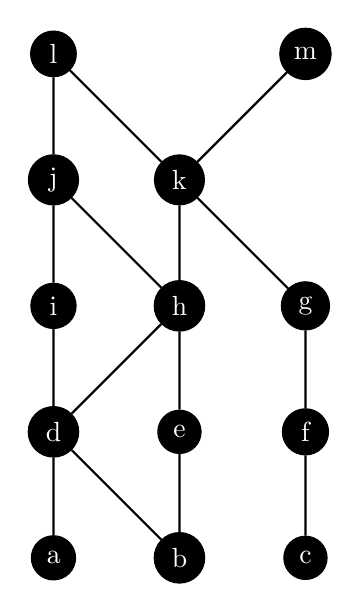
\begin{tikzpicture}[scale=0.8]
      \tikzstyle{node} = [draw,circle,fill=black,text=white]

      \def\nodes{a,b,c,d,e,f,i,h,g,j,k}
      \foreach \n/\p
      [count=\i from 0,
      evaluate= \i as \x using {2*Mod(\i,3)},
      evaluate= \i as \y using {2*int(\i/3)}]
      in \nodes {
        \node[node](\n) at (\x,\y) {\n};
      }
      \node[node](l) at (0,8) {l};
      \node[node](m) at (4,8) {m};

      \draw[thick,-] (a) -- (d) -- (i) -- (j) -- (h) -- (d) -- (b) -- (e) -- (h) -- (k) -- (l) -- (j);
      \draw[thick,-] (c) -- (f) -- (g) -- (k) -- (m);
      
    \end{tikzpicture}
  \end{minipage}
  \begin{minipage}{.65\textwidth}
    \begin{parts}
    \part[2] Find the maximal elements.
    \part[2] Find the minimal elements.
    \part[1] Is there a greatest element? If so, what is it?
    \part[1] Is there a least element? If so, what is it?
    \part[2] Find all upper bounds of $\{a,b,c\}$.
    \part[1] Find the least upper bound of $\{a,b,c\}$, if it exists.
    \part[2] Find all lower bounds of $\{f,g,h\}$.
    \part[1] Find the greatest lower bound of $\{f,g,h\}$, if it exists.
    \end{parts}
  \end{minipage}
  \begin{solution}
    % Write your solutions here
    \begin{parts}
    \part m, l
    \part a, b, c
    \part none
    \part none
    \part l, m, k
    \part k
    \part none
    \part none
    \end{parts}
  \end{solution}
  
\end{questions}

\end{document}

%%% Local Variables:
%%% mode: latex
%%% TeX-master: t
%%% End:
